\section{Topologie des éspaces métriques}
\begin{definition}
    .
    \begin{enumerate}
        \item Un ensemble $U \subset  E$ est ouvert si $\forall x \in U$ $\exists \delta > 0$ tel que $B(x, \delta) \subset U$.
        \item Un ensemble $F \subset E$ est fermé si $E \setminus F$ est ouvert, i.e $\forall x \in E \setminus F$ $\exists \delta > 0$ tel que $B(x, \delta) \subset E\setminus F$
    \end{enumerate}
\end{definition}
\begin{figure}[H]
    \centering
    \begin{subfigure}{0.45\textwidth}
        \centering 
        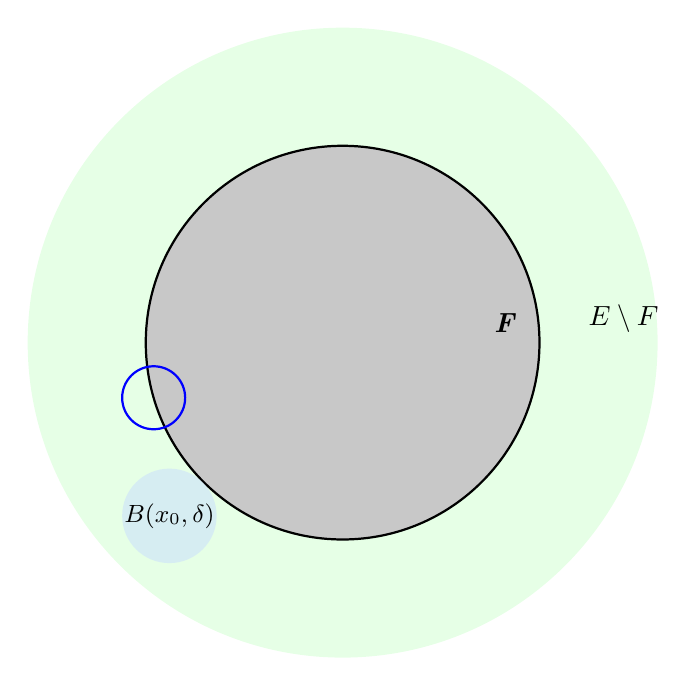
\begin{tikzpicture}
            % Define colors
            \definecolor{lightgreen}{RGB}{230, 255, 230}
            \definecolor{lightblue}{RGB}{200, 220, 255}
            \definecolor{darkgreen}{RGB}{0, 128, 0}

            % Large background circle
            \fill[lightgreen] (0, 0) circle (4cm);

            % Main circle
            \draw[thick, fill=lightgray] (0, 0) circle (2.5cm);
            \node[above right] at (1.8, 0) {\textbf{\textit{F}}};
            \node[above right] at (3, 0) {$E\setminus F$};

            % Small blue circle
            \draw[blue, thick] (-2.4, -.7) circle (0.4cm);

            % Highlighted area for excluded point
            \fill[lightblue, opacity=0.5] (-2.2, -2.2) circle (0.6cm);
            \node (_) at (-2.2, -2.2){\small $B(x_0, \delta)$};
        \end{tikzpicture}
        \caption{Un ensemble fermé\\
            \textit{À la borne, il est impossible de trouver une boules qui appartient à $F$, car il est impossible d'avoir une boule ouverte de  $r = 0$. Exemple: circle bleu foncé}\\
            \textit{Pour tout point dans $E \setminus F$ on peut trouver une boule ouverte}
        }
    \end{subfigure}
    \hfill
    \begin{subfigure}{0.45\textwidth}
        \centering
        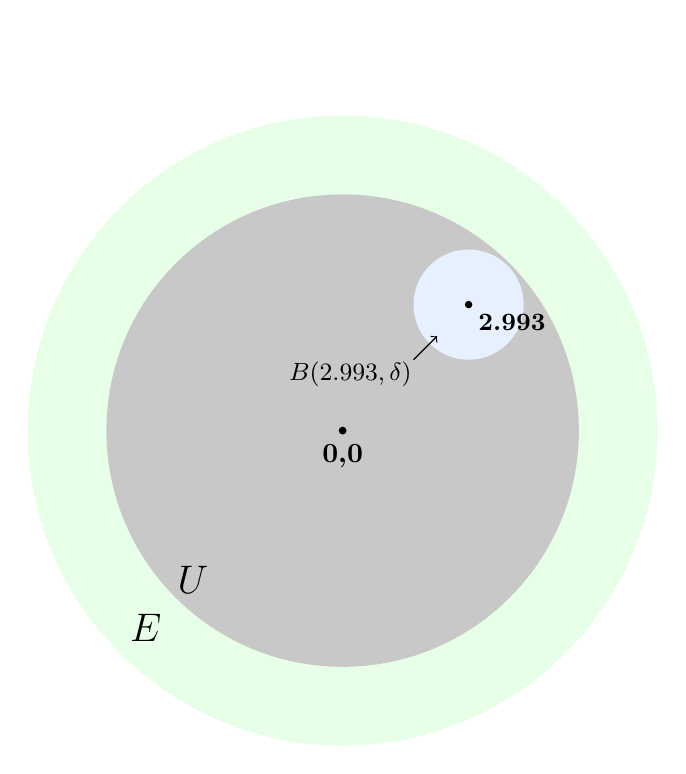
\begin{tikzpicture}
            % Define colors
            \definecolor{lightblue}{RGB}{230, 240, 255}
            \definecolor{lightgray}{RGB}{200, 200, 200}
            \definecolor{darkgreen}{RGB}{0, 128, 0}
            \definecolor{lightgreen}{RGB}{230, 255, 230}

            % Draw large circle
            \fill[lightgreen] (0, 0) circle (4cm);
            \fill[lightgray] (0, 0) circle (3cm);

            % Draw small circle
            \fill[lightblue] (1.6, 1.6) circle (0.7cm);
            \draw[fill=black] (1.6, 1.6) circle(0.4mm);
            \node[below right] at (1.6, 1.6) {\textbf{\small 2.993}};

            \draw[->] (0.9, 0.9)--(1.2, 1.2);
            \node[below left] (_) at (1, 1){\small $B(2.993, \delta)$};
            % Add points and labels
            \node[fill=black, circle, inner sep=1pt, label=below:{\textbf{0,0}}] at (0, 0) {};

            % Add text
            \node[right] at (1, 5) [align=left, text=darkgreen] {
                };
            \node (_) at (-1.9, -1.9){\Large $U$};
            \node (_) at (-2.5, -2.5){\Large $E$};
        \end{tikzpicture} 
        \caption{Un ensemble ouvert\\
            \textit{
                pour tout point pres de la borne
                on peut trouver une boule
                infiniment petite avec des
                points autour ce point inclu dans $U$.
            }
        }

    \end{subfigure}
    \caption{Démonstration des espaces ouverts et fermés}
\end{figure}
